\documentclass[11pt]{article}

\usepackage[margin=1in]{geometry}
\usepackage{amsmath,amssymb,amsthm}
\usepackage{mathtools}
\usepackage{stmaryrd} % \llbracket \rrbracket for the coalition bracket
\usepackage{booktabs}
\usepackage{graphicx}
\usepackage{hyperref}
\usepackage{enumitem}

\theoremstyle{definition}
\newtheorem{definition}{Definition}[section]
\theoremstyle{plain}
\newtheorem{theorem}{Theorem}[section]
\newtheorem{proposition}[theorem]{Proposition}
\newtheorem{corollary}[theorem]{Corollary}
\theoremstyle{remark}
\newtheorem{remark}[theorem]{Remark}

% proof-status tags: kernel-proved in i-orca, empirical, or open
\newcommand{\proved}{\textsc{[proved, i-orca]}}
\newcommand{\empirical}{\textsc{[empirical]}}
\newcommand{\open}{\textsc{[open]}}

\newcommand{\HH}{\mathcal{H}}
\newcommand{\RR}{\mathbb{R}}
\newcommand{\inner}[2]{\langle #1,\, #2\rangle}
\newcommand{\Uframe}{U}
\newcommand{\Gram}{G}
\newcommand{\Vh}{V_{\mathrm{head}}}
\newcommand{\Vt}{V_{\mathrm{tail}}}
\newcommand{\Sh}{S_{\mathrm{head}}}
\newcommand{\St}{S_{\mathrm{tail}}}
\newcommand{\umax}{u_{\max}}

\title{\textbf{Projective Incidence Calculus}\\[0.3em]
\large A semiring-weighted incidence algebra for the transformer decode,\\
its frozen-model geometry, and its learnable frame}
\author{}
\date{Draft --- companion to \texttt{spec/PIC\_SPEC.md} v0.3.1}

\begin{document}
\maketitle

\begin{abstract}
We give an algebraic account of the transformer next-token decision as a \emph{semiring-weighted
incidence calculus over a continuous inner-product geometry}---\emph{Projective Incidence Calculus}
(PIC). Propositions (tokens) are points $U_v$ in a residual space $\HH=\RR^d$; sources (per-layer
contributions, or learned rules) are vectors $d_j$; the incidence of a source on a proposition is the
inner product $\inner{d_j}{U_v}$; and the decision aggregates incidences through a commutative semiring
selected by a temperature $T$. At $T=1$ the semiring is the log-semiring and PIC \emph{is} the forward
pass (softmax over summed logits); as $T\to0$ it is the tropical (max-plus) semiring and PIC is the
geometry of margins, Laguerre power diagrams, and a head/tail decode certificate, the two ends joined
by Maslov dequantization. PIC separates the \emph{frame} (intrinsic geometry of $\{U_v\}$: Gram
coherence, Welch floor, packing capacity) from the \emph{decode} (margins, participation ratio,
multiplicity, evaluated in the chosen semiring). This separation organizes a three-part program:
analysis reads the decode off a frozen frame (a runtime that reconstructs the model's decode exactly),
verification proves two-sided packing bounds on the structures (a machine-checked corpus), and learning
holds the decode fixed while \emph{retraining the frame}. We state the calculus, its semiring family,
and the load-bearing theorems---each tagged as machine-proved, empirical, or open---and we cast the
learning problem as frame optimization under explicit soundness invariants.
\end{abstract}

\section{Introduction}

A transformer computes a next-token distribution by projecting a residual vector onto an unembedding
matrix and taking a softmax. Read literally this is a single linear map followed by a normalization; but
the residual vector is itself an \emph{additive} object---a sum of per-layer attention and MLP writes
plus the embedding---so the decode logit of token $v$ decomposes as a \emph{sum of inner products}, one
per contributing block. We take this decomposition as primitive and ask what algebra it lives in. The
answer is a semiring-weighted incidence calculus: tokens are propositions carrying geometric directions,
blocks are sources casting weighted votes, and the decision is the semiring aggregate of those votes.

The payoff of naming the algebra is that three otherwise-separate activities become facets of one
object. \emph{Analysis} of a frozen model is evaluation of the calculus in the log-semiring. With the
final normalization folded into the sources the decomposition is algebraically exact, and a decomposing
runtime reproduces the model's decode decision at every position measured (\S\ref{sec:calculus}).
\emph{Verification} is proving structural bounds---how many tokens a frame can decode, how many rules can
write the logits, what interference overpacking forces---and these are theorems about the calculus's
structures, machine-checked in a kernel. \emph{Learning} is the recognition that the frame is a free
parameter: one can hold the decode semantics fixed and deform the geometry so that more structure becomes
retrievable. PIC is the shared vocabulary that lets a definition in one activity be a hypothesis in
another.

This paper defines PIC (\S\ref{sec:core}--\S\ref{sec:calculus}), separates frame from decode
(\S\ref{sec:sep}), collects the proved theorems as a two-sided packing picture (\S\ref{sec:thm}), and
casts frame learning as constrained optimization (\S\ref{sec:learn}). Throughout we tag each claim
\proved{} (machine-checked), \empirical{} (measured), or \open{}.

\section{Core structures}\label{sec:core}

\begin{definition}[Frame and Gram kernel]
Let $V$ be a finite set of \emph{propositions} (tokens), $|V|=n_p$, and let $\HH=\RR^d$ be the residual
space. A \emph{PIC frame} is a map $\Uframe:V\to\HH$, $v\mapsto U_v$. It induces the \emph{Gram kernel}
$\Gram(v,w)=\inner{U_v}{U_w}$ and, after row normalization $\bar U_v=U_v/\lVert U_v\rVert$, the
\emph{cosine Gram} $\rho(v,w)=\inner{\bar U_v}{\bar U_w}$.
\end{definition}

The Gram kernel supplies the continuous, non-truth-functional overlap between propositions: tokens are
not independent atoms but directions with measurable coherence.

\begin{remark}[What the decode cannot see]\label{rem:gauge}
Three transformations leave every coalition decision, every margin and the full softmax unchanged:
\begin{itemize}[nosep]
  \item a common translation $U_v\mapsto U_v+h$, since each coalition's score on every token shifts by
        the same $\inner{\sum_{j\in P}d_j}{h}$;
  \item a common bias shift;
  \item a joint orthogonal change of basis of $\{U_v\}$ and $\{d_j\}$.
\end{itemize}
Rescaling the frame and the biases together, $(U,b)\mapsto(\alpha U,\alpha b)$ with $\alpha>0$, preserves
decisions and acts as a temperature change. Rescaling $U$ alone with fixed nonzero biases does not: with
$r=1$, $U=(1,0)$, $b=(0,2)$, the second token wins, but after $U\mapsto3U$ the first wins. Independent per-token
rescaling $U_v\mapsto\sigma_vU_v$ does \emph{not} preserve decisions in general. The cosine Gram, coherence
and frame potential are not translation-invariant. They are properties of a chosen \emph{representative}
of the frame, such as the centred frame $U_v-\operatorname{mean}_wU_w$, not of decoder behaviour, and a
change in them counts as a behavioural change only once that representative is fixed. The name
``projective'' refers to this direction reading of the frame, the cosine Gram being invariant under
positive per-vector rescaling. It is not an invariance of the decode.
\end{remark}

\begin{definition}[Sources, incidence, monomial, polynomial]\label{def:agg}
A \emph{source set} $S$ ($|S|=J$) assigns to each source $j$ a contribution $c_j:V\to R$ valued in a
semiring carrier $R$. The \emph{residual reading} fixes a vector $d_j\in\HH$ per source and sets the
\emph{incidence} $c_j(v)=\inner{d_j}{U_v}$. The two semiring operations play different roles:
\emph{$\otimes$ combines sources within a token}, giving a \emph{monomial}
\[
  L(v)=\Bigl(\bigotimes\nolimits_{j\in S} c_j(v)\Bigr)\otimes b_v=\sum_{j\in S}\inner{d_j}{U_v}+b_v
  \qquad(\text{$T$-independent});
\]
while \emph{$\oplus_T$ combines tokens}, giving the decode \emph{polynomial}
\[
  Z_T=\bigoplus\nolimits_{T,\,v\in V} L(v)
      =\bigoplus\nolimits_{T,\,v\in V}\ \bigotimes\nolimits_{j\in S} c_j(v)\otimes b_v .
\]
\end{definition}

Thus each token is a monomial and the decode is a $(\oplus_T,\otimes)$ polynomial whose monomials are the
tokens and whose variables are the sources---the tropical-polynomial picture of a ReLU network. The
decision reads off $Z_T$: at $T\to0$, $Z_0=\max_v L(v)$ and the decode is $\arg\max_v L(v)$; at $T=1$,
$Z_1=\operatorname{logsumexp}_v L(v)$ and $p(v)=\exp(L(v)-Z_1)$. The monomials are shared across $T$; only
$\oplus_T$ changes (Lemma~\ref{lem:tinv}).

In the transformer instance, the sources are the \emph{DLA blocks}: an $n_\ell$-layer model has $n_b=2n_\ell+1$
blocks (one attention and one MLP/expert write per layer, plus the embedding), and $d_j$ is block $j$'s
additive contribution to the residual at the decode position. The incidence $c_j(v)=\inner{d_j}{U_v}$ is
precisely the per-block contribution a decomposing runtime emits, and its source-sum reconstructs the
model's decode logit.

\paragraph{Native notation.} PIC borrows its carriers (semiring, Gram kernel, Welch bound, power
diagrams) so as to inherit their theorems, but three things are native and get their own notation. The
\emph{incidence arrow} $j\triangleright v:=\inner{d_j}{U_v}$ names the one new primitive---provenance as
an inner product in a learnable frame. The \emph{coalition bracket}
$\llbracket P\rrbracket(v):=\bigotimes_{j\in P}(j\triangleright v)$ is the partial monomial of a coalition
$P\subseteq S$ (no $T$: sources add). The \emph{decision turnstile} and its margin-indexed form are
\[
  P\vdash v\ :\Longleftrightarrow\ \llbracket P\rrbracket(v)-\max_{w\neq v}\llbracket P\rrbracket(w)\ >\ 0,
  \qquad
  P\vdash_\gamma v\ :\Longleftrightarrow\ \llbracket P\rrbracket(v)-\max_{w\neq v}\llbracket P\rrbracket(w)\ \ge\ \gamma
  \quad(\gamma>0)
\]
(``coalition $P$ decides $v$'', respectively ``\dots\ with margin $\ge\gamma$''; $P\vdash_\gamma v$
implies $P\vdash v$). The unsubscripted turnstile is \emph{strict}: a tie decides nothing. This is
exactly the kernel predicate \texttt{decides} (\texttt{PIC\_Core.thy}) that the irreducibility theorems of
\S\ref{sec:thm} quantify over. The turnstile collapses the decision regimes to one line each:
\emph{retrieved} $\exists j.\ \{j\}\vdash v$; \emph{composed} $S\vdash v$ but
$\forall j.\ \neg(\{j\}\vdash v)$; \emph{irreducible} $S\vdash v$ and
$\forall P\subsetneq S,P\neq\emptyset.\ \neg(P\vdash v)$. These are not a trichotomy. Given $S\vdash v$,
retrieved and composed are complementary. Irreducible is a subclass: for $|S|\ge2$ it implies composed,
and for $|S|=1$ it coincides with retrieved.

The turnstile reads the coalition bracket only, \emph{without} the bias $b_v$, again matching the kernel
definition. $S\vdash v$ therefore coincides with ``the model strictly decodes $v$'' exactly when $b\equiv0$,
which is the case for most transformer unembeddings. When $b\neq0$, adjoin the bias as one more source:
append a coordinate carrying $b_v$ to each $U_v$ and a source $d_{\mathrm{bias}}$ equal to the matching unit vector.
Then $\llbracket S\cup\{b\}\rrbracket(v)=L(v)$, and every statement below applies to the augmented source set.

\section{The semiring family}\label{sec:semiring}

PIC is parameterized by a temperature $T\ge 0$ selecting a commutative semiring
$(R_T,\oplus_T,\otimes,0,1)$ with a fixed product $\otimes=+$ (incidences along a coalition add) and a
$T$-dependent sum:
\[
  a\oplus_T b \;=\; T\,\log\!\bigl(e^{a/T}+e^{b/T}\bigr),
  \qquad
  a\oplus_T b \xrightarrow[\;T\to 0^+\;]{} \max(a,b).
\]

\begin{center}
\begin{tabular}{@{}llll@{}}
\toprule
$T$ & semiring & $a\oplus_T b$ & reading \\
\midrule
$1$ & log-semiring & $\log(e^a+e^b)$ & probabilistic incidence $\to$ softmax \\
$\to 0^+$ & tropical (max-plus) & $\max(a,b)$ & argmax, margins, power diagrams \\
general & deformed & $T\log\sum e^{\cdot/T}$ & temperature-controlled decoding \\
\bottomrule
\end{tabular}
\end{center}

The two ends are joined by \emph{Maslov dequantization}: the probabilistic calculus (the model in
operation) and the geometric calculus (the proofs) are limits of one deformation, not different objects.

\begin{definition}[The complete semiring]\label{def:semiring}
For each $T\ge0$, $R_T=(R,\oplus_T,\otimes,\mathbf{0},\mathbf{1})$ has carrier $R=\RR\cup\{-\infty\}$,
sum $a\oplus_T b=T\log(e^{a/T}+e^{b/T})$ with $\oplus_0:=\max$, product $a\otimes b=a+b$, sum identity
$\mathbf{0}=-\infty$, and product identity $\mathbf{1}=0$. It satisfies the semiring axioms: $(R,\oplus_T)$
is a commutative monoid with identity $-\infty$; $(R,\otimes)$ is a commutative monoid with identity $0$;
$\otimes$ distributes over $\oplus_T$; and $\mathbf{0}$ annihilates ($-\infty\otimes a=-\infty$). It is
commutative, and idempotent exactly at $T=0$ ($a\oplus_0 a=a$ but $a\oplus_1 a=a+\log 2$)---the algebraic
difference between geometry and probability.
\end{definition}

\noindent The distributive law $a\otimes(b\oplus c)=(a\otimes b)\oplus(a\otimes c)$ rewrites a
sum-of-maxes (a ReLU stack) as a max-of-sums (a tropical polynomial). \emph{What is machine-checked}
\proved{} (\texttt{TropicalSemiring.thy}) is the $T=0$ case over the finite carrier $\RR$:
associativity, commutativity and idempotence of $\oplus_0=\max$; associativity, commutativity and the
identity $0$ of $\otimes=+$; and both distributive laws. The formalization has no $-\infty$. The
$\oplus$-identity $\mathbf{0}=-\infty$ and annihilation $-\infty\otimes a=-\infty$ hold by the
definitions on $\RR\cup\{-\infty\}$ but are \emph{not} kernel-checked. Nor is anything for $T>0$, where
the laws are the elementary log-domain identities (e.g.\
$a+T\log(e^{b/T}+e^{c/T})=T\log(e^{(a+b)/T}+e^{(a+c)/T})$). For $T>0$ they also follow from the
isomorphism $x\mapsto e^{x/T}$ onto the ordinary semiring $(\RR_{\ge0},+,\times)$, so every
$R_T$ with $T>0$ is the same semiring up to isomorphism. The one algebraically distinct member is $T=0$.

\section{PIC as a calculus}\label{sec:calculus}

\paragraph{Syntax.} Sources are weighted facts, and a \emph{coalition} $P\subseteq S$ is a derivation
body whose incidences combine under $\otimes$. In the decode fragment each proposition $v$ has exactly
\emph{one} derivation: the full coalition $S$, together with the bias. So $\otimes$ is the only operation
inside a proposition. As in Definition~\ref{def:agg}, $\oplus_T$ ranges over the \emph{competing
propositions}, the alternative answers to the decode query. It does not range over alternative derivations of
one $v$.

\paragraph{Semantics.} Semiring annotation in the style of Green--Karvounarakis--Tannen: the annotation of
$v$ is $L(v)\in R_T$. The Gram kernel supplies the continuous overlap that a Boolean annotation lacks.
Because $v$ has a single derivation, its provenance polynomial is the single monomial $L(v)$. $\oplus_T$
enters one level up, at the query, as the partition $Z_T=\bigoplus_{T,v}L(v)$. This is the log-partition
at $T=1$ and the decode value at $T=0$. A genuine $\oplus$ over \emph{alternative derivations of the same
atom}, the case the provenance framework is built for, arises only in recursive or multi-derivation
programs (\S\ref{sec:learn}), not in the one-step decode. Proposition~\ref{lem:tinv} does not extend to
such programs (Remark~\ref{rem:tinv-scope}). The decision predicates are
\emph{not} semiring values: the margin $m(t)=L(t)\oslash\bigoplus_{0,\,w\neq t}L(w)$ needs the
$\otimes$-inverse, which exists because max-plus on $\RR$ is a semifield, and it always uses the
tropical sum. The turnstile is therefore a tropical side condition on annotations at every $T$.

\paragraph{Decision rules} (in the native turnstile of Definition~\ref{def:agg}).
\begin{itemize}[nosep]
  \item \emph{Aggregate:} $L(v)=\llbracket S\rrbracket(v)\otimes b_v$; decode $\arg\max_v L(v)$.
  \item \emph{Retrieved:} $\exists j\in S.\ \{j\}\vdash v$ (a singleton decides, so $\mu_t\ge1$;
        $\{j\}\vdash_\gamma v$ is the margin-$\gamma$ strengthening).
  \item \emph{Composed:} $S\vdash v$ but $\forall j\in S.\ \neg(\{j\}\vdash v)$ (no singleton; $\mu_t=0$).
  \item \emph{Irreducible:} $S\vdash v$ and $\forall P\subsetneq S,P\neq\emptyset.\ \neg(P\vdash v)$.
\end{itemize}

\paragraph{Soundness anchors.}
\begin{itemize}[nosep]
  \item \emph{Log-semiring $\Rightarrow$ transformer.} The sources are block writes with the final
        normalization \emph{folded in}. Let $s$ be the inverse scale, computed once from the full
        pre-norm residual and frozen, and $\theta$ the learned gain. For RMSNorm, $\tilde d_j=s\,\theta\odot d_j$.
        For LayerNorm, $\tilde d_j=s\,\theta\odot(d_j-\operatorname{mean}(d_j))+\mathbf 1_{j=\mathrm{embed}}\,\beta$:
        centring is per block (the means add up to the full-residual mean), and the norm bias $\beta$ is
        assigned by convention to the embedding block. Then $\sum_j\tilde d_j$ is the normed residual. Both
        conventions affect coalition attribution. Three claims must be kept apart.
        \begin{enumerate}[nosep]
          \item \emph{Algebraic reconstruction.} Given the frozen norm, the incidence sum equals the model
                logit by linearity. The linear part is \texttt{logit\_is\_residual\_reading} \proved{}; the
                fold is an exact interface convention for the given input.
          \item \emph{Numerical logit error.} This is not currently reported.
          \item \emph{Decision agreement} \empirical{}. The reconstructed argmax over the emitted candidate
                set (target plus a fixed number of top competitors) equals the model's at every measured position,
                across rotary, NeoX, mixture-of-experts and latent-attention architectures. This is what
                ``reconstruction $1.00$'' measures. It does not by itself establish equal logits or equal
                distributions.
        \end{enumerate}
        With the norm scale and downstream blocks frozen, $\llbracket P\rrbracket$ for a proper coalition is
        a \emph{direct-effect} quantity, not the model's behaviour when $S\setminus P$ is ablated.
  \item \emph{Tropical $\Rightarrow$ power diagram.} As $T\to0$, $\arg\max_v \inner{r}{U_v}+b_v$ is
        Laguerre (power-diagram) cell membership over sites $\{U_v\}$ with weights
        $\omega_v=\lVert U_v\rVert^2+2b_v$, under the convention
        $\arg\min_v\lVert r-U_v\rVert^2-\omega_v$. The capacity theorems of \S\ref{sec:thm} are the geometry
        of that diagram.
\end{itemize}

\noindent The two anchors are consistent only because of a fact native to the $T$-family:

\begin{proposition}[Decode temperature-invariance]\label{lem:tinv}
For every $T>0$, $\arg\max_v L(v)$ is the same token, equal to the tropical ($T\to0$) decoder; only the
normalized confidence $p_T(v)=\exp\bigl((L(v)-Z_T)/T\bigr)$ and the partition $Z_T=\bigoplus_{T,v}L(v)$
depend on $T$.
\end{proposition}
\begin{proof}
The monomials $L(v)=\llbracket S\rrbracket(v)\otimes b_v$ carry no $T$ (sources combine by $\otimes=+$).
$T$ enters only the cross-token aggregator $\oplus_T$, which is strictly order-preserving in each
argument with $\arg\max=(\oplus_0)$-selector; hence the $\arg\max$ of the fixed vector $(L(v))_v$ is
$T$-independent. $\oplus_T$ reweights how much the winner beats the field, never which token wins.
\end{proof}

\begin{remark}[Scope: one derivation per answer]\label{rem:tinv-scope}
The proof uses the fact that each answer's score is a single $T$-free monomial. The proposition fails
once $\oplus_T$ also merges alternative derivations \emph{within} an answer. Suppose answer $A$ has two
score-$0$ derivations and answer $B$ one score-$0.5$ derivation. At $T=1$, $A$ scores $\log2\approx0.69$
and wins; at $T\to0$, $A$ scores $0$ and $B$ wins.
\end{remark}

This is the rigorous bridge between the anchors: the \emph{proofs} run at $T\to0$ (tropical margins,
power-diagram capacity, head/tail) and the \emph{model} runs at $T=1$ (softmax), yet they decode the same
token because they share the monomials. Every margin/decode theorem of \S\ref{sec:thm} proved tropically
therefore transfers verbatim to the operating model's greedy (argmax) decision. The $T$-dependent part
is the normalized confidence $p_T$ and its entropy. Margins $m(t)$ contain no $T$.

\section{Encode, frame, decode}\label{sec:sep}

PIC is a sandwich of three roles: the \emph{encoder} writes the residual, the \emph{frame} is the shared
dictionary, and the \emph{decoder} reads it out. The encode side has an explicit model
(machine-checked, \texttt{PIC\_Core.thy}).

\begin{definition}[Encoder]\label{def:enc}
A PIC encoder fixes a finite rule set $K$, fixed write directions $a:K\to\HH$, and input-dependent gates
$g:K\to(X\to\RR)$. On input $x$ the residual is the gated sum $\operatorname{enc}(x)=\sum_{k\in K}g_k(x)\,a_k$,
and the logit is $L(v;x)=\inner{\operatorname{enc}(x)}{U_v}+b_v=\sum_{k\in K}g_k(x)\inner{a_k}{U_v}+b_v$.
\end{definition}

This expresses any transformer block: a block's residual write is $W_{\mathrm{out}}\cdot(\text{input
vector})$---fixed output columns $a_k$ gated by an input coefficient $g_k(x)$---for MLP and attention
alike. The gate $g_k(x)$ is left \emph{uninterpreted}: PIC formalizes the linear write/read algebra
($\inner{a_k}{U_v}$ is rule $k$'s incidence) and leaves the nonlinear gate as the un-modelled forge tax,
so the encoder sharpens rather than enlarges the calculus. Three facts are proved \proved{}: the forward
pass is one PIC term ($L(v;x)=\sum_k g_k(x)\inner{a_k}{U_v}+b_v$); every encoded residual lies in
$\operatorname{span}\{a_k\}$ of dimension $\le\min(|K|,d)$ (routing rank, now a property of the encoder---
\S\ref{sec:thm}); and every fixed-input slice \emph{is} a source model (Def.~\ref{def:agg}) with
$d_k=g_k(x)a_k$. The remaining two roles split every other quantity:

Every other PIC quantity is either \emph{frame-side} (a function of $\{U_v\}$ alone---intrinsic,
label-free) or \emph{decode-side} (a function of the aggregate $L$ and a target, evaluated in the chosen
semiring).

\paragraph{Decode-side.}
margin $m(t)=L(t)-\max_{v\neq t}L(v)$;\quad
participation ratio $\mathrm{PR}=\bigl(\sum_j|c_j(t)|\bigr)^2/\sum_j c_j(t)^2$ over the target incidences
(the effective number of sources with sizeable target incidence);\quad
multiplicity $\mu_t=\#\{j:\arg\max_v c_j(v)=t\}$ (unanimity; with a tie-broken argmax it can count a
source that ties $t$ and so does not satisfy $\{j\}\vdash t$);\quad
ambiguity $\eta^2$ (between/total variance of candidate firing on the lowest-margin slice).

\begin{remark}[Architecture-fair PR]
When sources carry a common-mode component identical across candidates (e.g.\ a LayerNorm/embedding
offset), it cancels in the argmax but inflates raw $\mathrm{PR}$. The discriminative count centres each
source across candidates first, $\mathrm{PR}\bigl((c_j(t)-\overline{c_j})_j\bigr)$; raw and centred agree
for RMSNorm frames and diverge for LayerNorm. Use the centred form for cross-architecture comparison.
\end{remark}

\begin{remark}[What PR does not measure]\label{rem:pr}
PR is not a sufficient-coalition size, in either direction. Take incidences over $(t,x,y)$ of
$c_a=(1,2,0)$ and $c_b=(0,-2,\tfrac12)$. The sum $(1,0,\tfrac12)$ decodes $t$, and no singleton does,
yet $\mathrm{PR}=1$. Conversely, many identical deciding sources give a large PR. PR is also not invariant
under re-decomposition, since splitting a source into $k$ equal parts inflates it without changing the
residual. PR describes participation under a fixed decomposition. Coalition sufficiency is the turnstile's
job.
\end{remark}

\paragraph{Frame-side.}
Gram coherence $\max_{v\neq w}|\rho(v,w)|$;\quad
frame potential $\mathrm{FP}=\operatorname{mean}_{v\neq w}\rho(v,w)^2$;\quad
Welch floor $W=(n_p-d)/\bigl(d(n_p-1)\bigr)$ for $n_p>d$, else $0$. Always $\mathrm{FP}\ge W$. Because FP
uses cosines, it depends only on the normalized directions $\bar U_v$, and its equality cases are
statements about them. For $n_p>d$, $\mathrm{FP}=W$ iff $\{\bar U_v\}$ is a unit-norm tight frame
(Benedetto--Fickus). Equiangularity is an additional condition: it is the equality case of the
\emph{max}-coherence bound. For $n_p\le d$, $W=0$ and $\mathrm{FP}=0$ iff the directions are pairwise
orthogonal, which does not require tightness on all of $\HH$. The ratio $\mathrm{FP}/W$ is defined only
for $W>0$. These quantities depend on the
frame representative (Remark~\ref{rem:gauge}).

\section{The two-sided packing theorems}\label{sec:thm}

The proved results split into a \emph{frame side} (how many tokens a geometry can decode) and a
\emph{generator side} (how many rules can write the logits, and what interference overpacking forces).
This split is not a coincidence: it is the \emph{two arities} of the decode polynomial $Z_T$ of
Definition~\ref{def:agg}. A $(\oplus,\otimes)$ polynomial has a monomial-count and a variable-rank, and
PIC bounds each---the frame side bounds the \textbf{monomials} (tokens that can be cleanly decoded, the
$\oplus$-arity) at $(1+2\umax/\gamma)^d$, the generator side bounds the \textbf{variables} (independent
sources, the $\otimes$-arity) at $\min(M,d)$. ``Two-sided packing'' is thus a simultaneous bound on a
polynomial's monomial-count and its variable-rank. Welch is the interference floor on \emph{both} sides.
The readouts are overpacked too: $n_p\gg d$, so $\mathrm{FP}(U)\ge W>0$ and the unembedding frame is in
superposition. On the generator side, overpacking provably forces routing cross-talk
(Theorem~\ref{thm:welch}). On the frame side, the only proved capacity bound is astronomically loose for
realistic $d$, so it is not what limits real models. A loose upper bound does not show that frame geometry
is non-binding, however. Whether frame coherence limits achievable margins is the open
coherence$\Rightarrow$margin question.

\subsection{Frame side: decode capacity (monomial count)}

Call $v$ \emph{$\gamma$-decodable} if some unit-ball residual $r$ ($\lVert r\rVert\le1$) makes it win by
margin $\gamma$: $\forall w\neq v,\ \inner{r}{U_w}+b_w+\gamma\le\inner{r}{U_v}+b_v$.

\begin{theorem}[Margin separation \proved{}]\label{thm:sep}
If $v$ and $w$ are both $\gamma$-decodable then $\gamma\le\lVert U_v-U_w\rVert$.
\end{theorem}
\begin{proof}[Proof sketch]
Add the two witness inequalities; the biases cancel, and Cauchy--Schwarz with $\lVert r_v-r_w\rVert\le2$
gives the bound. (Machine-checked in \texttt{DecodeCapacity.thy}.)
\end{proof}

\begin{corollary}[Head capacity]\label{cor:cap}
\textup{(i)} \proved{} Any set $V'\subseteq V$ of $\gamma$-decodable tokens is a $\gamma$-code:
$\lVert U_v-U_w\rVert\ge\gamma$ for distinct $v,w\in V'$ (\texttt{head\_capacity}).
\textup{(ii)} Hence, by the classical volume-packing argument, $|V'|\le(1+2\umax/\gamma)^d$ with
$\umax=\max_v\lVert U_v\rVert$. The argument: disjoint radius-$\gamma/2$ balls about the points of $V'$
fit inside the ball of radius $\umax+\gamma/2$.
\end{corollary}

\noindent Only part (i) is kernel-checked. The cardinality bound (ii) is a standard textbook step that the
i-orca corpus does not formalize: the Lebesgue-measure argument is absent, so (ii) must not be cited as
\proved{}. This is the cell-capacity half. The bound is astronomically loose for realistic $d$. That
looseness shows the bound is not the constraint, not that frame geometry never constrains margins.

\subsection{Generator side: routing rank and Welch interference (variable rank)}

$M$ rules write logit adjustments along fixed readout vectors $\{a_1,\dots,a_M\}$ through
input-dependent gates $g_k(x)$.

\begin{theorem}[Routing superposition \proved{}]\label{thm:rank}
$\sum_{i\in I}g_i\,a_i\in\operatorname{span}(a_I)$ and $\dim\operatorname{span}(a_I)\le|I|$. Every rule
adjustment lives in a subspace of dimension $\le\min(M,d)$; superposition is forced when the number of
routing decisions exceeds $M$.
\end{theorem}

\begin{theorem}[Routing Welch \proved{}]\label{thm:welch}
For $n$ unit-norm routing features in $M$ coordinates,
$\sum_{i\neq j}\inner{f_i}{f_j}^2\ge n(n-M)/M$, strictly positive exactly when $n>M$. Cross-talk-free
routing requires $M\ge n$.
\end{theorem}

\begin{remark}[The missing link \open{}]
The step ``routing interference $\Rightarrow$ margin degradation'' is \emph{not} a kernel theorem.
Trained models pack features at $\approx$ the Welch floor with healthy margins; the coherence-to-margin
implication is measured and mild, not proved.
\end{remark}

\subsection{The decode certificate and its robustness}

With $\operatorname{decode}(L,V')=\max_{v\in V'}L(v)$ for a token set $V'\subseteq V$:

\begin{theorem}[Head/tail certificate \proved{}]\label{thm:headtail}
$\operatorname{decode}(L,\Vh\cup\Vt)=\max(\operatorname{decode}(L,\Vh),\operatorname{decode}(L,\Vt))$, and if
$\operatorname{decode}(L,\Vt)\le\operatorname{decode}(L,\Vh)$ then the full decode equals the head decode and
its argmax lies in $\Vh$. If instead the head does not dominate, the decision lies in the tail---the
explicit, uncertified residue.
\end{theorem}

\begin{theorem}[Margin certificate, threshold tight \proved{}]\label{thm:margin}
If $|L'(v)-L(v)|\le\delta$ for all $v$ and $m(t)>2\delta$, then $t$ remains the strict argmax under $L'$.
The constant $2\delta$ is tight (a $m(t)=2\delta$ token can be tied by a $\delta$-perturbation), and the
certificate is silent for $m(t)\le2\delta$---exactly the small-margin residue.
\end{theorem}

\noindent Note what Theorem~\ref{thm:headtail} partitions: \emph{tokens} ($\Vh,\Vt\subseteq V$), i.e.\ the
monomials of $Z_0$. The empirical sparse-circuit finding is about something else: a per-position head of
a few late-layer \emph{blocks} reproduces the decode \empirical{}. That finding partitions \emph{sources}
and needs Theorem~\ref{thm:margin} instead. Split $S=\Sh\sqcup\St$, and let
$L_{\mathrm{head}}(v)=\llbracket\Sh\rrbracket(v)+b_v$ be the head-only logit. Suppose the tail's contribution
is within $\delta$ of a common offset $\kappa$ on every candidate, $|\llbracket\St\rrbracket(v)-\kappa|\le\delta$.
Then $L=L_{\mathrm{head}}+\llbracket\St\rrbracket$ is a $\delta$-perturbation of $L_{\mathrm{head}}+\kappa$,
which has the same argmax and the same margins as $L_{\mathrm{head}}$. So if the head's margin exceeds $2\delta$, its decision is the model's.
This is an immediate instance of Theorem~\ref{thm:margin}, not separately kernel-checked. Tokens whose head
margin is $\le2\delta$ are the source-side residue.

\subsection{Irreducibility}

For a composition matrix $c:\text{sources}\times\text{outcomes}\to\RR$, $S$ \emph{decides} $t$ if
$\sum_{j\in S}c(j,v)<\sum_{j\in S}c(j,t)$ for all $v\neq t$; $\mu_0$ holds if no singleton decides $t$;
$S$ is \emph{irreducible} for $t$ if it decides $t$ and no proper nonempty subset does.

\begin{theorem}[$\mu_0\nRightarrow$ irreducible \proved{}]\label{thm:irr}
There is an explicit instance with $\mu_0$ (no single source decides $t$) in which a proper pair already
decides $t$; and a separate explicit fully-irreducible triple. Hence ``no singleton decides'' does not
imply ``all sources needed''.
\end{theorem}

This is the precise statement of $\mu_t=0\neq\text{irreducible}$: low multiplicity is necessary but not
sufficient for genuine irreducibility. Whether a composed token is irreducible under \emph{every}
admissible frame---the real necessity question---is \open{}.

\section{Frame learning as constrained optimization}\label{sec:learn}

Fix the decode semantics (log-semiring $L$, softmax) and optimize the frame $U$---equivalently, deform
the Gram kernel---so that more propositions become retrievable:
\[
  \mathcal{L}(U)=\underbrace{\mathrm{NLL}(L;t)}_{\text{decode, data}}
  +\;\lambda_m\underbrace{\operatorname{ReLU}\!\bigl(\gamma^\star-m(t)\bigr)}_{\text{decode, margin}}
  +\;\lambda_f\underbrace{\mathrm{FP}(U)}_{\text{frame, structure}} .
\]
The decode-side terms anchor the aggregate to the targets and push the worst-competitor margin past
$\gamma^\star$; the frame-side term decorrelates propositions toward the Welch floor. A
Generate--Gate--Refine loop wraps the gradient step: \emph{generate} candidate sources (random or
frame-aligned, or real DLA blocks loaded through the analysis seam), \emph{gate} them by the PIC
diagnostics ($\eta^2$, activation variance, firing decorrelation), \emph{refine} by a step on
$\mathcal{L}$.

\paragraph{Soundness invariants.} The loop should preserve: (S1) \emph{decode soundness}---the refined
frame still realizes a valid log-semiring decoder on held data; (S2) \emph{margin monotonicity}---the
certified margin mass $\#\{t:m(t)>2\delta\}$ of Theorem~\ref{thm:margin} does not decrease; (S3)
\emph{frame admissibility}---$\mathrm{FP}(U)\ge W$ is structural, so a report must target $\mathrm{FP}/W\to1$
and never claim to beat the floor. These are natural targets for learning-side soundness theorems.

\paragraph{What is established \empirical{}.} On synthetic benchmarks no theory-guided knob
(frame-regularization, allocation/targeting, propose-score-select, coherence-regularization) beats plain
SGD on $\mathcal{L}$; PIL training \emph{is} gradient descent on the frame, cheap only as a shallow head
on frozen sources. The win that exists is \emph{retraining the frame/subspace}---the movable side of the
boundary---rather than fitting an encoder into a frozen dictionary, consistent with the verification-side
result that frozen compression hits a $\Theta(d)$ floor a rank-bottlenecked retrained update clears.

\paragraph{The logic-programming reading.} Structurally PIC is a semiring-weighted logic program with
two strata.
\begin{itemize}[nosep]
  \item \emph{The decode stratum is non-recursive and uses aggregates.} Its atoms are source facts
        $\mathrm{src}(j)$ weighted by $j\triangleright v$, and decision atoms $\mathrm{dec}(v)$. Let
        $A=\{j:\mathrm{src}(j)\in I\}$. The model's decision is the \emph{full}-coalition aggregate:
        $\mathrm{dec}(v)$ holds iff $A\vdash v$. Because $\vdash$ is strict, this derives at most one
        decision atom, and none on a tie. The emitted program's \texttt{max}-aggregate \texttt{decide} is the
        argmax relation instead, which derives every maximizer. The two agree exactly under a
        unique-maximum precondition; otherwise a selection policy (such as the model's tie-break) must be
        stated. Sub-coalition
        sufficiency is a separate witness relation,
        $\mathrm{wit}(P,v)\Leftrightarrow P\subseteq A\wedge P\vdash v$. Opposing singletons can witness
        different tokens at once, so an existential rule
        ``$\exists P\subseteq A.\ P\vdash v\Rightarrow\mathrm{dec}(v)$'' would record witnesses, not the
        decode. No $\mathrm{dec}$ or $\mathrm{wit}$ atom occurs in a body. The stratum is evaluated once,
        after the layer stratum (stratified aggregation), and is not a monotone Horn operator.
  \item \emph{The layer stratum is where recursion enters.} Its atoms $(\ell,x)$ say ``the residual at
        layer $\ell$ is $x$'', the embedding is a fact, and each layer is a clause
        $(\ell{+}1,\mathrm{step}_\ell\,x)\Leftarrow(\ell,x)$. Its least model is exactly the forward
        trajectory \proved{} (\texttt{PIC\_Forward.thy}, \texttt{lfp\_is\_trajectory}). The decode logits are
        the frame read-out of its final-layer fact \proved{} (\texttt{lfp\_decode\_logits}), and the
        decode stratum is evaluated on top.
\end{itemize}
The semiring chooses the aggregation: $T=0$ gives Viterbi/min-cost evaluation, $T=1$ gives logsumexp,
and Boolean gives classical Datalog. Logsumexp over derivations is not by itself ProbLog's possible-world
semantics: overlapping explanations share facts, and summing them double-counts. Algebraic ProbLog needs
extra machinery for this, which PIC does not supply. PIC's one native move is that the fact weights are
\emph{derived from geometry}, $j\triangleright v=\inner{d_j}{U_v}$, rather than given.

Demand closure, $\operatorname{lfp}(\operatorname{restrict}\,\mathcal T\,D)=\operatorname{lfp}\mathcal T\cap D$ for a
monotone, demand-closed consequence operator $\mathcal T$, is proved \proved{} (\texttt{PIC\_Logic.thy},
\texttt{demand\_restrict\_lfp}; also \texttt{ProvableOpt\_Common.thy}). It gives the soundness of the
magic-sets/demand optimization for any stratum whose operator is a monotone set operator on atoms. That
includes the layer program, where values ride as atom arguments. The \texttt{sum}/\texttt{max} aggregates of
the decode stratum are not monotone set operators, so a demand theorem for the weighted aggregate
evaluation itself is \open{}. The likely route is stratified: the decode stratum is non-recursive
and runs on the layer stratum's fixed output, so it would suffice to show that each aggregate reads only
demanded atoms. This is not attempted. The margin certificate (Theorem~\ref{thm:margin}) bounds how far a clause
weight may drift before an answer flips. The frame/decode separation acts as the type discipline:
frame-side clauses (what overlaps what) and decode-side queries (margins, multiplicity).

\section{An empirical parameter the proofs do not pin down}\label{sec:tau}

Let $\tau^\star$ be the effective rank that the packing exponent would take in practice, in place of the
ambient $d$. What we measure is a different quantity: $r_{\mathrm{eff}}$, the common-mode-centred
participation ratio of decode blocks. Identifying $r_{\mathrm{eff}}$ with $\tau^\star$ is itself \open{}.
PR counts participation under one chosen decomposition and changes under source splitting
(Remark~\ref{rem:pr}), so it is not a geometric rank without a separate argument. The findings below are
therefore about $r_{\mathrm{eff}}$. The natural conjecture $r_{\mathrm{eff}}\approx\min(e^{H},d)$, with $H$ the
next-token entropy, is \emph{refuted} on a fourteen-model sweep to 72B (Pythia 14m--12b, Qwen
0.5B--72B; decision agreement $1.00$ throughout). The architecture-fair count $r_{\mathrm{eff}}$ \emph{anti}-correlates
with $e^{H}$ (Pearson $-0.54$) and associates with \emph{capacity} (hidden Spearman $+0.63$, $n_b$/depth
$+0.58$); the ratio $r_{\mathrm{eff}}/e^{H}$ climbs monotonically $0.07\to1.74$ across the ladder---larger,
more confident models use \emph{more} effective blocks, not fewer. These pooled correlations mix two families
whose within-family trends diverge, so the within-family statements below are the reliable ones.

But there is \emph{no clean functional form}: it is \textbf{architecture-dependent}
(Figure~\ref{fig:arch}A). Within Pythia,
$r_{\mathrm{eff}}\approx(0.4\text{--}0.5)\,n_b$ and grows with depth ($8\to30$ as $n_b:13\to73$); within
Qwen, $r_{\mathrm{eff}}$ is \emph{flat} ($\sim11\text{--}17$) while the block \emph{fraction} shrinks
$0.27\to0.10$ from 0.5B to 72B. (The once-tempting ``$\approx$12 scale-invariant blocks'' reading was a
Qwen raw-PR artifact---Qwen's raw PR is flat $7.7\text{--}13.8$ to 72B, while Pythia's grows to $37$.) A
genuine but modest \emph{within-model} effect survives (higher-entropy tokens use somewhat more blocks;
Spearman $\approx0.2\text{--}0.47$ in capable models)---a second-order grain, not the cross-model driver.
The same architecture split shows up in a \emph{wholly independent, causal} probe---the convergence depth
$k^\star/n_\ell$ (the smallest layer prefix whose recompute already reproduces the decode), which declines with
scale in Pythia but not Qwen (Figure~\ref{fig:arch}B)---so it is a property of the models, not an artifact
of the attribution measure. So $r_{\mathrm{eff}}$ is capacity-associated rather than entropy-bound, with
\emph{no universal law} across architectures; its functional form is \open{}. We keep it as the sharpest example of the discipline the
tags enforce: a plausible law, measured to 72B, and reported by what the data support---including the
architecture split---rather than by what would have been tidy.

\begin{figure}[t]
  \centering
  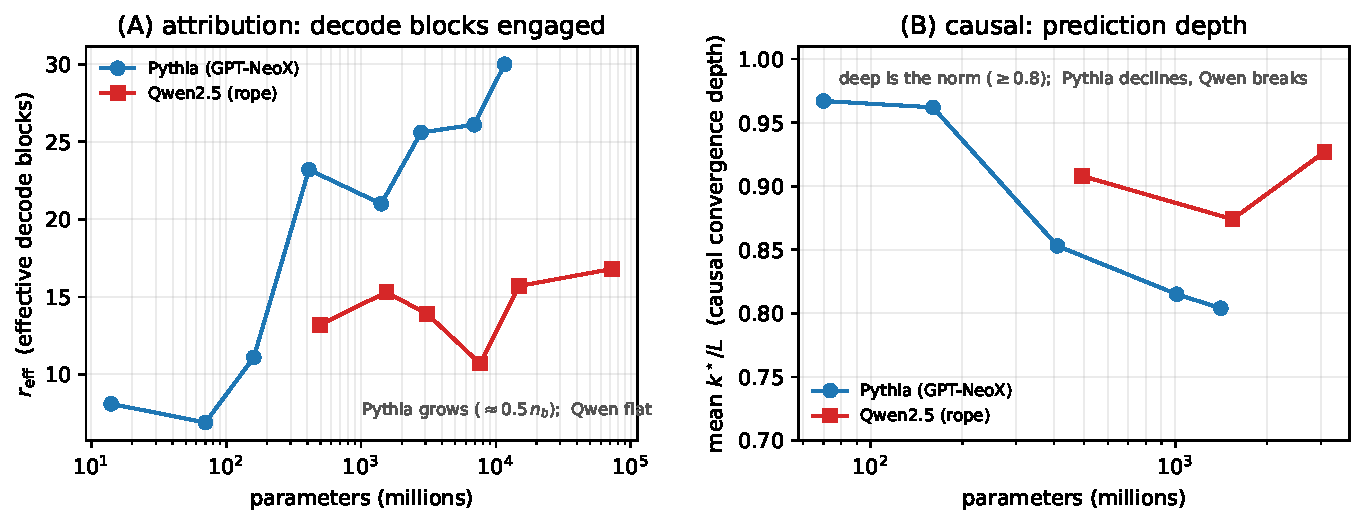
\includegraphics[width=\linewidth]{figures/arch_dependence.pdf}
  \caption{Two independent probes of how much of the model the next-token decode engages, both splitting
  Pythia from Qwen. \textbf{(A)} \emph{Attribution}: the effective number of decode blocks
  $r_{\mathrm{eff}}$ across the $\tau^\star$ sweep (14m--72B, reconstruction $1.00$): within Pythia it
  grows ($\approx0.5\,n_b$), within Qwen it is flat ($\sim$11--17) as the block fraction shrinks to
  $0.10$. \textbf{(B)} \emph{Causal}: the convergence depth $k^\star/n_\ell$ (\texttt{--converge-depth}) ---
  the smallest layer prefix whose recompute reproduces the decode. Deep computation is the norm
  ($k^\star/n_\ell\geq0.8$); Pythia's fraction declines with scale while Qwen's does not. That two unrelated
  measures --- one attributional, one causal --- agree on the architecture split is the load-bearing
  point: there is no universal scaling law for decode engagement.}
  \label{fig:arch}
\end{figure}

\section*{Provenance of claims}
\proved{} statements are machine-checked in the i-orca Isabelle corpus
(\texttt{tropical/\{TropicalSemiring,HeadTail,DecodeCapacity,RoutingRank\}.thy},
\texttt{superposition/\{Welch,RoutingWelch,Superposition\}.thy},
\texttt{pic\_core/\{PIC\_Core,PIC\_Logic,PIC\_Forward\}.thy},
\texttt{provable\_opt/ProvableOpt\_Common.thy}, \texttt{fieldrun/separation/Separation.thy}), all under
\texttt{i-orca/examples/}. A \proved{} tag covers exactly the statement kernel-checked there. Classical
steps layered on top, such as the volume-packing count of Corollary~\ref{cor:cap}(ii) and the extended-real
semiring laws of \S\ref{sec:semiring}, are marked as not kernel-checked where they occur.
\empirical{} statements are measured by the fieldrun runtime and the pil experiments.
\open{} statements are flagged hypotheses. See \texttt{spec/PIC\_SPEC.md} for the operational
definitions and file-level pointers.

\end{document}
